
\chapter{Data Exploration, Data Preprocessing and Feature Selection}
\thispagestyle{plainbottom}
The performance of machine learning algorithms depends on the type of data. When the data is analyzed and transformed appropriately then meaningful results can be obtained from our Machine learning algorithms. So, the main aim of this chapter is to explore, analyze and preprocess the data that will be used for our models. In the first section, the different datasets used for our analysis are explained and different aspects of the datasets has been discussed. There are there different datasets that have been used for our research, the main one is provided by three different psychological labs in SU. Then, in the second section, various preprocessing steps to transform the actual dataset have been discussed and in the final section, discussion about the results obtained from different feature selection algorithms for various parts of our research.
\section{Data Exploration}
The data that has been used for our research has been provided by the labs `Russo', `Antshel' and `Kates'. It has taken them over 10 years to collect this data and consists of information related to 369 children. Each of these children have different developmental disorders and the Venn diagram in figure \ref{fig:Venn} shows how the disorders are distributed. The age of children in this data is from 3 years to 18 years and the average age is 10 years.  Also,  the age at which the test has been taken by each subject is given. However, 70\% of the subjects don't have the age at which 
they have taken the test. There are a total of 98 features in the given data. The data consists of features where the children have taken three different parent-oriented reviews. 

\begin{figure}
\centering
   {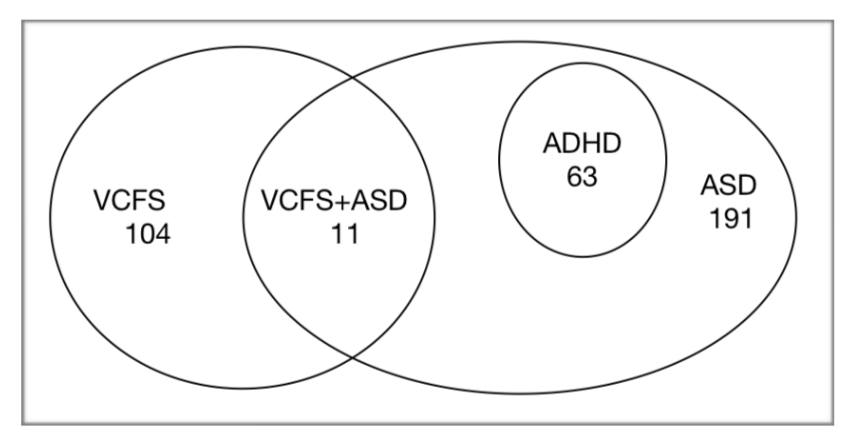
\includegraphics[width=0.6\textwidth]{Figures/Figure_3_1.png}}
  \caption{Venn Diagram of the division of diagnosis}
  \label{fig:Venn}
\end{figure}

However, not all children have taken all three parent-oriented review, figure \ref{fig:Reviews} gives details of how many children among the 369 have taken each of the tests. It can be observed that there only 48\% of subjects who have taken the VINE while majority have taken the ADI and the BASC.

\begin{figure}
\centering
  {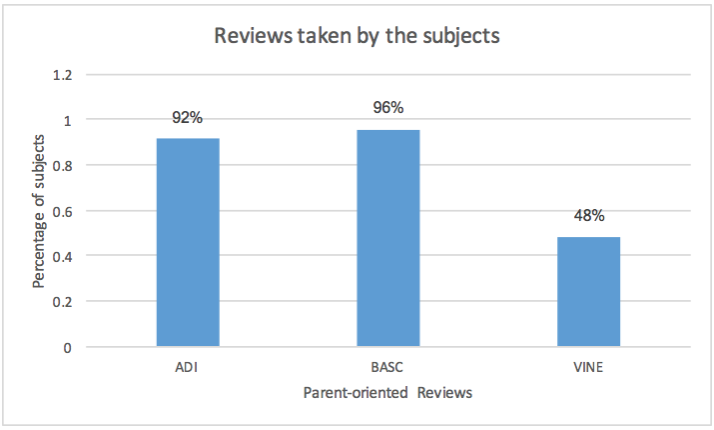
\includegraphics[width=0.6\textwidth]{Figures/Figure_3_2.png}}
  \caption{Reviews taken by subjects in percentage}
  \label{fig:Reviews}
\end{figure}
The verbal IQ, non-verbal IQ and full scale IQ of the subjects is measured, and the range of IQ is from 40 to 160 with a mean IQ of 100. Out of the 369 children, there are 252 male children which constitutes 68\% of the data and there are 117 female children which constitutes the rest 31\% of the data. The figure \ref{fig:Reviews2} gives information on how many children have taken the reviews based on gender. If our models were to be trained on this data, then it could be observed that models would be biased towards males over females as they are more dominant the dataset. On the male subjects, the classifier had an accuracy of 96.03\%, ROC Area value of 0.997 and F-measure of 0.959. On the other hand, the classifier gave an accuracy of 88.03\%, ROC Area value of 0.972 and F-measure of 0.851. Therefore, most of our models predict the diagnosis labels in the subgroup data for male subjects with a better accuracy of 7\% when compared to female subjects.
\begin{figure}
\centering
  {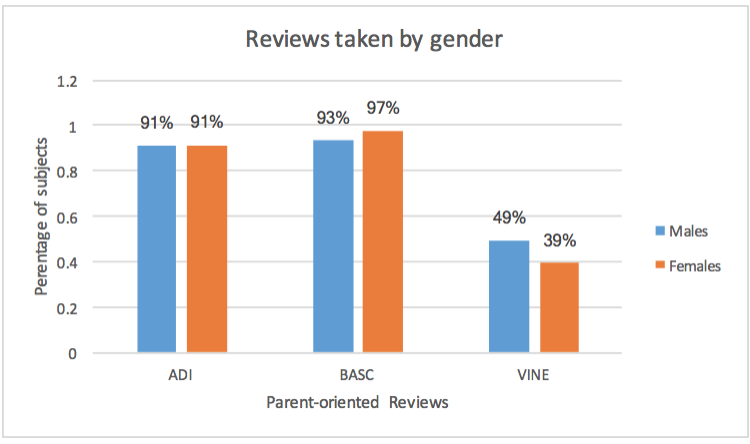
\includegraphics[width=0.6\textwidth]{Figures/Figure_3_3.png}}
  \caption{ Parent-oriented reviews taken by gender}
  \label{fig:Reviews2}
\end{figure}

Also, further analysis of the actual data shows that for certain subjects, certain feature values are missing. When the person has taken a parent-oriented review, then certain questions in the review were missing. So, features of each parent-oriented having missing values have been analyzed. It could be observed that, from subjects who have taken the VINE parent-oriented review, none of the feature values were missing. The features of ADI parent-oriented review and BASC parent-oriented review which had missing values are shown in figures\ref{fig:ADI} and \ref{fig:BASC} respectively. When considering the missing features for ADI, the missing sections have been considered as the parents have failed to fill a particular section of the review. Even though the missing values of individual sections is as high as 45\%, it can be seen that the missing values of each of the four domains is very low(A-2\%, BV-4\%, BNV-8\%, C-13\%, D-3\%). This shows that particular sub sections of the review are not filled, but overall sections in the review are filled. So, in the case of ADI, the missing features when handled accurately can avoid model over-fitting due to outliers. When we analyze the features of BASC, it was observed that only 4 out of 16 features had missing values. The feature `Adaptability' had 20\% of its features missing and the other features had very low percentage of missing values.
\begin{figure}
\centering
  {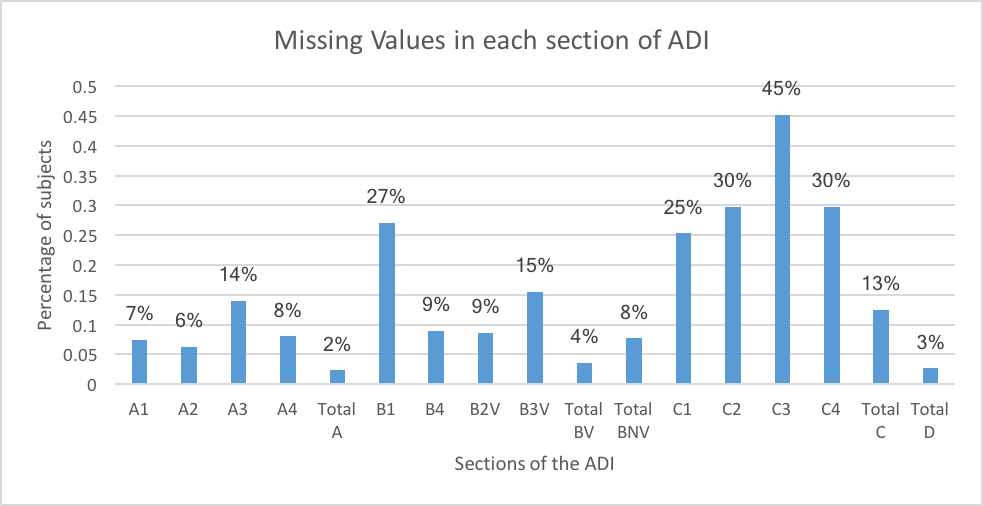
\includegraphics[width=0.6\textwidth]{Figures/Figure_3_4.png}}
  \caption{Analyzing missing values of features in ADI}
  \label{fig:ADI}
\end{figure}
\begin{figure}
\centering
  {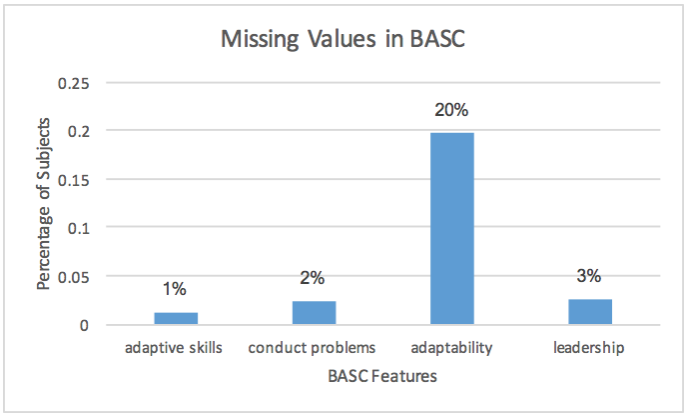
\includegraphics[width=0.6\textwidth]{Figures/Figure_3_5.png}}
  \caption{Analyzing missing values of features in BASC}
  \label{fig:BASC}
\end{figure}
\newline
In our research, when analyzing about the comorbid disorders ASD and ADHD, the `ABIDE' and `ADHD-200' datasets have also been used along with our actual dataset. These datasets have phenotypes and f(MRI) images of the brain and for our research the phenotypes aspect of the dataset has been taken. When analyzing how IQ is effecting the comorbidity of ASD and ADHD, the subjects from these datasets who have been diagnosed with ASD and ADHD were added to our dataset. The main reason behind this is that our dataset doesn’t contain any children with only ADHD. To keep our data balanced subjects were selected randomly from 539 ASD individuals and 285 ADHD individuals.
\section{Data Preprocessing}
This is one of the most important steps of the data mining process. The presence of noisy, irrelevant and unreliable data makes it difficult for knowledge discovery during the training phase of machine learning. Some of the preprocessing steps applied to our data to make it suitable for our training phase are as follows: 
\begin{itemize}
	\item Data Transformation- This is the process of converting the given data into a desired format. The most common transformation technique applied to our dataset is the conversion of  categorical features. Most of the data transformation steps that have been applied are given below and these steps are necessary for using the machine learning algorithms from sklearn package:
	\begin{compactenum}
		\item The feature `Sex' is converted to 1 (indicates male) and 0 (indicates female).
		\item All other feature columns whose attribute values are ‘YES/NO’ will be converted to 1  (for yes) and 0 (for no) .
		\item The target column `Diagnosis' is mapped to labels as follows: \begin{compactenum}\item ASD is 0 
\item ADHD+ASD is 1 
\item VCFS+ASD is 2 
\item VCFS is 3  \end{compactenum}
Also, when individual developmental disorders are studied or when we study comorbidity, the target column will be changed according. For example when analyzing ASD, all the children diagnosed with ASD will be mapped to 1 and others will be mapped to 0. Similar mapping will be done during different parts of our research.
	\end{compactenum}
Some parts of our research use machine learning algorithms from WEKA, for this purpose, the transformation technique used is to convert the data types of ADI features from numeric to nominal. Therefore, by applying these transformation techniques the data types will be correctly interpreted by the machine learning algorithms that will be used for our analysis.
\item Data Reduction- This is the process of reducing the given data to include only the necessary columns. Our data consists of many unique identifiers and unnecessary columns. By doing this, over-fitting of the data during the training phrase can be avoided. Over-fitting of our model means that our model is too closely fit to the data and it makes the model more complex than necessary.  The following are the steps taken to reduce our feature set:
	\begin{compactenum}
    \item The columns- `Subject ID', `Lab', `BASC', `VINE', `ADI' and `ADIAUTISM' are removed from the dataset and are not used by the model for prediction. The feature `ADIAUTISM' is a direct indicator of whether a child has ASD or not, hence it needs to be removed from our data. Now, the total number of features/variables on which the model will be trained is 92. 
	\item Further more, the columns which have totals for the ADI test have also been removed from the dataset, as these columns contain redundant feature information and are just simply sum of previous features. 
	\item Also, the age attribute has been condensed from four, that is three columns `ADI Age`, `BASC Age` and `VINE Age` remain. For the children who don’t have these age, their actual age from the `Age(Years)` is considered to be the age when the reviews were taken by the children. 
    \end{compactenum}
After applying the data reduction techniques on our data, the final number of features on which the training will be done is 73 including the target column `Diagnosis'. In WEKA, this step can be carried out using the Remove attribute feature. Hence, with the help of this step, our models will be able to generalize over our data.
\item Data Cleaning- It is a process of detecting, correcting or removing inaccurate instances from our data. The most important task in our data cleaning step is handling missing values. As seen in the data exploration section, most of our features have missing values. While handling missing values in our data, the structure of our data should not be effected, that is they should not become noise or outliers of our data. Hence, it is important that each features of our feature set are handled differently so that the structure of our actual data is maintained. The following are the steps as to how the missing values are handled:
\begin{compactenum}
\item Handling missing values for IQ test features- The PRI, VCI and FSIQ column’s missing values are replaced with the mean value which is 100. This has not affected the mean value of the dataset, so it is a good idea to replace missing values with 100. 
\item Handling missing values for ADI parent-oriented review features- The scores for ADI features/variables ranges from 0 to 2. In this case, the missing values are replaced with a 0 because this indicates not present. When the value is missing it is safe to assume that that the symptom is not present in the children than making any other assumptions and leading to false outcomes. 
\item Handling missing values for BASC parent-oriented review features- The scores have a mean of 50 and the standard deviation of 10. When the values are 70 it means it is critical. So, for this test the values are going to be replaced with the mean that is 50. For any value below 50, the score is not to be considered, hence, the missing values in the dataset are replaced with 50. 
\item Handling missing values for VINE parent-oriented review features- The scores are standard and the missing values are going to be replaced with 0. This is because most subjects don't have the VINE gets scores and the subjects that have taken the VINE tests have the results without any missing values. 
\end{compactenum}
\end{itemize}
After the preprocessing of the data, the model is trained on the modified features. The next sections discuss the training steps and the results obtained after training the model. Also, before training the model out of the 73 features, the features best used to train the model are selected so that the model can be trained correctly with these important features.

\section{Feature Selection}
Feature selection also known as variable selection is the process of selecting a subset of features from our given data. The different feature selection algorithms used in our research are LASSO regression\nomenclature{LASSO}{Least Absolute Shrinkage and Selection Operator}, ReliefF and Recursive Feature Elimination
\nomenclature{RFE}{Recursive Feature Elimination}. The LASSO regression method that selects subset of variable when there is highly correlated predictors in the data, as in our dataset.  On the other hand, ReliefF is a noise tolerant and robust algorithm which is independent of variable dependencies. While RFE uses an elimination process to select a subset of features recursively from our data. One or all of these feature selection algorithm have been applied on different aspects of our research and the results obtained are discussed in the following sections.

\subsection{Subgroup Diagnosis}
As part of our research, initially, predictions are done on the actual data sample. Feature selection algorithms are used on the preprocessed data which has 73 features and the best 5 features are selected. The root mean squared error \nomenclature{RMSE}{Root Mean Square Error} is used to analyze the performance of our feature selection models. Also, the best features are selected by doing 10-fold cross validation, that is at each fold the best features are taken and then finally best 5 features are found using a weighted average. ReliefF algorithm was not applied to our data to select best features as there are multi class labels in our data and ReliefF works well for binary classifiers. The RMSE for LASSO and RFE is 0.6837 and 0.66575. Both of these models have similar RMSE and hence, it can be said that these models are have similar performance measures when selecting the best features. However, LASSO has selected features from BASC and VINE, whereas RFE has selected features from ADI and are shown in table \ref{table:Subgroup}. So, there are no convergent features selected by these two algorithms.
%%table 3.1
\begin{table}[h]
\begin{center}
\begin{tabular}{|p{7 cm}|p{8 cm}|}
\hline
\textbf{LASSO} & \textbf{Recursive Feature Elimination}\\
\hline \hline
\begin{enumerate}
\item Performance IQ
\item Activities of Daily Living
\item Vineland daily living
\item Adaptability
\item Vineland Composite 
\end{enumerate}  & \begin{enumerate}
\item Criteria for repetitive behaviors and stereotyped patterns
\item Criteria for qualitative impairments in reciprocal social interaction
\item Quality of social overtures
\item Offers comfort
\item Inappropriate questions or statements
\end{enumerate} \\
\hline
\end{tabular}
\end{center}
\caption{Best 5 variables by different feature selection algorithm for Subgroup Diagnosis}
\label{table:Subgroup}
\end{table}

\subsection{Comorbid Developmental Disorders}
There are two groups of comorbid disorders that are analyzed in our research. The first one is ASD and ADHD comorbidity and the other group is ASD and VCFS comorbidity. The actual data is divided to separate ASD and ASD+ADHD to analyze the comorbid disorders ASD and ADHD. This data consists of 254 subjects who have been diagnosed with ASD, out of which 63 subjects have ADHD as well. This data consists of 190 males and 64 females where 53 males  and 10 females have ADHD along with ASD. For analyzing ASD and VCFS comorbidity, the data used consists of 115 subjects diagnosed with VCFS and 11 have ASD as well. Even though there are 49 females and 55 males, this data is more balanced than other data that we have used so far. The best features for both these comorbidities is analyzed in this section. 
%table 3.2
\begin{table}[h]
\begin{center}
\begin{tabular}{|p{5 cm}|p{5 cm}|p{6 cm}|}
\hline
\textbf{ReliefF} & \textbf{LASSO} & \textbf{Recursive Feature \newline Elimination}\\
\hline \hline
\begin{enumerate}
\item Vineland socialization
\item Attention problems
\item Performance IQ
\item Vineland\newline Communication
\item Vineland Composite
\end{enumerate}  & \begin{enumerate}
\item Vineland socialization
\item Quality of \newline social overtures
\item Offering to share
\item Inappropriate questions or statements
\item Attention problems
\end{enumerate} & \begin{enumerate}
\item Quality of social overtures
\item Inappropriate questions or statements
\item Abnormality of development evident at or before 36 months
\item Criteria for Qualitative impairments in reciprocal\newline social interaction
\item Conventional/Instrumental Gestures
\end{enumerate} \\
\hline
\end{tabular}
\end{center}
\caption{Best 5 variables by different feature selection algorithm for ASD and ADHD comorbidity}
\label{table:comorbidASD}
\end{table}

For ASD and ADHD comorbid disorders, the best 5 features from the three feature selection algorithms are given in table \ref{table:comorbidASD}. The RMSE for LASSO, ReliefF and RFE is 0.289, 0.493 and 0.224 respectively. So, it shows that RFE and LASSO are performing better than ReliefF feature selection algorithm as they have lower RSME values. The LASSO feature selection algorithm has selected features from all three parent-oriented reviews and the RFE feature selection algorithm as selected all variables from ADI review. While the ReliefF has selected variables from BASC and VINE. It can be seen that there are convergent variables in the LASSO feature selection algorithm.

The best features for ASD and VCFS comorbidity selected when applying the three feature selection algorithms is given in table \ref{table:comorbidVCFS}. The RMSE for LASSO, ReleifF and RFE is 0.0093, 0.9484 and 0.07 respectively. By the observed RMSE values, it can be observed that LASSO and RFE high performance and ReliefF has poor performance. another observation made after looking at the features is that there no convergent features from different parent-oriented reviews. In fact, the LASSO selects the features from BASC, ReliefF from VINE and RFE from ADI. The only convergent feature is the `Performance IQ' selected by both LASSO and ReliefF.
%Table 3.3
\begin{table}[h]
\begin{center}
\begin{tabular}{|p{5 cm}|p{5 cm}|p{6 cm}|}
\hline
\textbf{LASSO} &\textbf{ReliefF} & \textbf{Recursive Feature \newline Elimination}\\
\hline \hline
\begin{enumerate}
\item Anxiety
\item Hyperactivity
\item Performance IQ
\item Conduct Problems
\item Depression
\end{enumerate}  & \begin{enumerate}
\item Verbal IQ
\item Vineland Composite
\item Performance IQ
\item Full Scale IQ
\item Vineland Daily Living
\end{enumerate} & \begin{enumerate}
\item Criteria for Repetitive behaviors and stereotyped \newline patterns
\item Repetitive use of objects or interest in parts of objects
\item Verbal Rituals
\item Criteria for Communication
\item Hand and Finger\newline mannerisms
\end{enumerate} \\
\hline
\end{tabular}
\end{center}
\caption{Best 5 variables by different feature selection algorithm for ASD and VCFS comorbidity}
\label{table:comorbidVCFS}
\end{table}

\subsection{Individual Developmental Disorders Diagnosis}
Our data consists of information related to three different developmental disorders that is ASD, VCFS and ADHD. For each of these disorders, the features are analyzed and the best features are found. The target label `Diagnosis' is converted to `ASD Diagnosis', `ADHD Diagnosis' and `VCFS diagnosis' for each of the disorders. Then, the 73 features preprocessed data is given as input to our feature selection algorithms and the best features for each developmental disorder are observed.
%Table 3.4-
\begin{table}[h]
\begin{center}
\begin{tabular}{|p{5 cm}|p{5 cm}|p{6 cm}|}
\hline
\textbf{LASSO} &\textbf{ReliefF} & \textbf{Recursive Feature \newline Elimination}\\
\hline \hline
\begin{enumerate}
\item Behavioral Symptoms
\item Performance IQ
\item Full Scale IQ
\item Adaptive Skills
\item Externalizing \newline problems
\end{enumerate}  & \begin{enumerate}
\item Activities of Daily\newline Living
\item Vineland \newline Communication
\item Vineland Composite
\item Vineland Daily Living
\item Functional \newline Communication 
\end{enumerate} & \begin{enumerate}
\item Criteria for Repetitive behaviors and stereotyped\newline patterns
\item Use of other's body to \newline communicate
\item Criteria for Qualitative impairments in reciprocal social interaction
\item Hand and Finger \newline mannerisms
\item Repetitive use of objects or interest in parts of \newline objects
\end{enumerate} \\
\hline
\end{tabular}
\end{center}
\caption{Best 5 variables by different feature selection algorithm for ASD}
\label{table:ASD}
\end{table}

The best features for distinguishing children with ASD from those who don't have it are given in table \ref{table:ASD}. The RMSE values for LASSO, RFE and ReliefF are 0.181, 0.218 and 0.523. This shows that LASSO and RFE are performing better than ReliefF due to the low RSME scores. LASSO selects the best features from the BASC parent-oriented review, ReliefF selects from both the BASC and the VINE parent-oriented review and RFE selects from ADI. Also, it can be observed that there is no overlap of features by all three feature selection algorithms.

%Table 3.5
\begin{table}[t]
\begin{center}
\begin{tabular}{|p{5 cm}|p{5 cm}|p{6 cm}|}
\hline
\textbf{LASSO} &\textbf{ReliefF} & \textbf{Recursive Feature \newline Elimination}\\
\hline \hline
\begin{enumerate}
\item Performance IQ
\item Full Scale IQ
\item Behavioral Symptoms
\item Adaptive Skills
\item Direct Gaze
\end{enumerate}  & \begin{enumerate}
\item Performance IQ
\item Vineland socialization
\item Vineland \newline communication
\item Vineland daily living
\item Vineland composite
\end{enumerate} & \begin{enumerate}
\item Inappropriate questions or statements
\item Quality of social overtures
\item Conventional/Instrumental Gestures
\item Criteria for Qualitative impairments in reciprocal\newline social interaction
\item Offers comfort
\end{enumerate} \\
\hline
\end{tabular}
\end{center}
\caption{Best 5 variables by different feature selection algorithm for ADHD}
\label{table:ADHD}
\end{table}

%Table 3.6
\begin{table}[t]
\begin{center}
\begin{tabular}{|p{5 cm}|p{5 cm}|p{6 cm}|}
\hline
\textbf{LASSO} &\textbf{ReliefF} & \textbf{Recursive Feature\newline Elimination}\\
\hline \hline
\begin{enumerate}
\item Hyperactivity
\item Criteria for Qualitative impairments in \newline reciprocal social interaction
\item Pronominal reversal
\item Vineland \newline Communication
\item Vineland Socialization
\end{enumerate}  & \begin{enumerate}
\item Activities of Daily Living
\item Functional \newline Communication 
\item Vineland \newline Communication
\item Vineland daily living
\item Vineland composite
\end{enumerate} & \begin{enumerate}
\item Criteria for Repetitive behaviors and stereotyped\newline patterns
\item Use of other's body to \newline communicate
\item Pronominal reversal
\item Neologisms/idiosyncratic language
\item Stereotyped Utterances \& delayed echolalia
\end{enumerate} \\
\hline
\end{tabular}
\end{center}
\caption{Best 5 variables by different feature selection algorithm for VCFS}
\label{table:VCFS}
\end{table}
The children with ADHD and those who don't have can be distinguished using the best features given in table \ref{table:ADHD}. The RMSE values for LASSO, RFE and ReliefF are 0.190, 0.201 and 0.407. The LASSO selects features from BASC, while the ReleifF selects from VINE and RFE selects from ADI. Even in this case there are no convergent parent-oriented reviews features except the Performance IQ feature. As the RMSE values are low for LASSO and RFE, the models are performing better than ReliefF.

For the developmental disorder VCFS, the RMSE values for LASSO, RFE and ReliefF are 0.189, 0.308 and 0.555. The best features selected by each of the three feature selection algorithms are given in table \ref{table:VCFS}. LASSO select features from all of the three parent-oriented reviews, while ReliefF selects from BASC and VINE. On the other hand, RFE selects from ADI. In this case, the convergent features are from ADI and VINE which are selected by LASSO.

When all of the feature selection algorithms are compared, it can be seen that RFE usually tends to select algorithms from the ADI parent-oriented review, while ReleifF selects mostly from VINE parent-oriented review and sometimes from BASC. LASSO is the only feature selection algorithm that has selected features from all three parent-oriented reviews. LASSO and RFE are both performing better than ReliefF. However, LASSO feature selection algorithm can be considered to be doing a better job as it has selected features from all three reviews. Also, LASSO assigns coefficients to each of the features and these coefficients can be negative or positive. It eliminates all the unimportant features by assigning them weights 0. Therefore, for most parts of our research only LASSO features have been used for our analysis.
